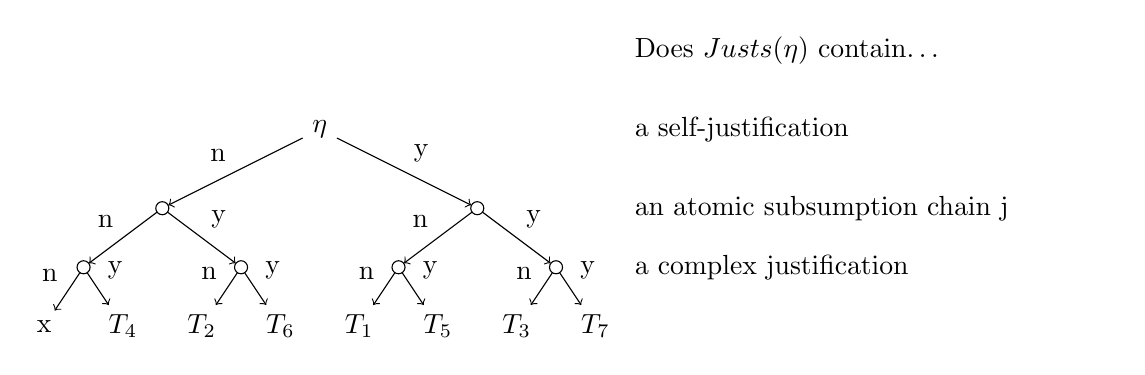
\begin{tikzpicture}[scale=1,->,auto=left]
  
%  \draw (-2,8.25) -- (6,8.25) -- (6,7.75) -- (-2,7.75) -- cycle;
% \draw (-2,7.5) -- (6,7.5) -- (6,7) -- (-2,7) -- cycle;
%  \draw (-2,8.25) -- (6,8.25) -- (6,7.75) -- (-2,7.75) -- cycle;
\node[align=left,text width=6cm] at (9,10) {Does $Justs(\eta)$ contain\ldots};
\node[align=left,text width=6cm] at (9,9) {a self-justification};
\node[align=left,text width=6cm] at (9,8) {an atomic subsumption chain j};
\node[align=left,text width=6cm] at (9,7.25) {a complex justification};
  
\node[draw=none] (root) at (2,9) {$\eta$};

\tikzstyle{every node} = [color=black,shape=circle,scale=0.5,draw]
  
\node (n) at (0,8)  {};
\node (y) at (4,8)  {};
\node (nn) at (-1,7.25)  {};
\node (ny) at (1,7.25)  {};
\node (yn) at (3,7.25)  {};
\node (yy) at (5,7.25)  {};

\tikzstyle{every node} = [draw=none]
\node[draw=none] (nnn) at (-1.5,6.5)  {x};

\node (nny) at (-0.5,6.5)  {$T_{4}$};	
\node (nyn) at (0.5,6.5)  {$T_{2}$};
\node (nyy) at (1.5,6.5)  {$T_{6}$};
\node (ynn) at (2.5,6.5)  {$T_{1}$};
\node (yny) at (3.5,6.5)  {$T_{5}$};
\node (yyn) at (4.5,6.5)  {$T_{3}$};
\node (yyy) at (5.5,6.5)  {$T_{7}$};



\draw (root) to node [swap]  {n} (n);
\draw (root) to node {y} (y);

\draw (n) to node [swap] {n} (nn);
\draw (n) to node {y} (ny);

\draw (nn) to node [swap]  {n} (nnn);
\draw (nn) to node {y} (nny);

\draw (ny) to node [swap]  {n} (nyn);
\draw (ny) to node {y} (nyy);

\draw (y) to node [swap]  {n} (yn);
\draw (y) to node {y} (yy);

\draw (yn) to node  [swap] {n} (ynn);
\draw (yn) to node  {y} (yny);

\draw (yy) to node [swap]  {n} (yyn);
\draw (yy) to node  {y} (yyy);


\end{tikzpicture}